\chapter{Allelic divergence in the polar diatom \textit{Fragilariopsis cylindrus}}
\label{chap:diatom}
\chaptermark{Allelic divergence in the polar diatom \textit{F. cylindrus}}

This chapter is based on a submitted scientific paper:

\vspace{5mm}

\textit{Mock, T., Otillar, R. P., Strauss, J., Allen, A. E., Dupont, C. L., Frickenhaus, S., ... Grigoriev, I. V. (Submitted). Extensive genetic diversity and differential bi-allelic expression in a Southern Ocean diatom. Nature.}

\vspace{5mm}

This project was a very large collaboration spanning many years to sequence the genome of the \textit{Fragilariopsis cylindrus} organism.
In order to clearly describe my work and set it in context, some work that was not performed by myself is described.
In particular, any work mentioned in the introduction is not my contribution to the work, but was completed by colleagues.
My contributions to the work are described in sections 4.2.2.1, 4.2.2.2, 4.2.2.3, 4.2.2.4, and the results section presents data that was the outcome of my work only.
In the discussion some further preliminary work is described. A figure showing this work is provided as an appendix, and this work was done jointly and equally between myself and a colleague.

\newpage

\section{Introduction}

\subsection{Sexual reproduction and recombination}

Sex as a mode of reproduction has a two-fold cost.
Firstly, most sexually reproducing species only have one gender capable of bearing offspring \parencite{DeVisser2007}.
Secondly, in sexually reproducing organisms, any individual will only contribute approximately half of its genetic information to each offspring; i.e. in diploid sexuals, gametes are haploid \parencite{Agrawal2001}.
In contrast, an asexually reproducing, clonal organism contributes all of its genetic information to each offspring, and every individual is typically capable of bearing young \parencite{Schlupp2010}.
This generalization applies to most sexual organisms however, there are exceptions. 
For example, not all sexually producing organisms have the two-fold cost problem. 
Yeasts are sexual organisms with two mating types and both types are capable of producing offspring.
In addition, a species of poecilids can reproduce through a process of gynogenesis; a process similar to asexual reproduction through parthenogenesis, but is distinct as the presence of sperm is required to stimulate egg development \parencite{Schlupp2010}.
Hybridisation has also given rise to a Hermaphroditic Cichlid individual which can self \parencite{Svensson2016}.
In addition, some species shuttle between asexual and sexual reproduction, and the frequency at which this happens directly affects the factors raised above.

All else being equal, an asexual species should outperform a sexual species over time because of its faster population growth rate.
However, sexual and asexual species do co-exist together, sometimes with similar fecundity \parencite{Schlupp2010}.
However, despite this, sexual reproduction is very widespread, especially among the eukaryotes.
These observations led researchers to think that the benefits of sexual reproductions must be evolutionary and lead to the production of offspring with benefits that outweigh to costs.
To summarize most of the commonly cited reasons sexual reproduction is maintained, it may be described as a mechanism, through which: 

\begin{enumerate}
\item Beneficial mutations can spread through a population more quickly.
\item Novel genetic combinations are generated.
\item Deleterious mutations can be purged or masked.
\end{enumerate}

These benefits are possible because sexual reproduction brings together into one individual, the chromatids (and alleles they contain) in the gametes of two parental individuals from separate genealogical lines (out-crossing).
In addition, when parental individuals generate gametes, meiotic recombination will result in new combinations of genes \parencite{Felsenstein1976}.
This in turn contributes to the generation of novel genetic (or rather, genotypic) variation.
As a result, two or more beneficial mutations from separate genealogical lines may occur together within the same individual, thus facilitating the spread of beneficial mutations through the population to fixation.

This is formalized by the Hill-Robertson effect \parencite{Hill1966}, and is demonstrated by considering two loci with the haplotype $A_2B_2$ with a fitness of $1$.
It is then assumed two mutants at both loci ($A_1B_2$, $A_2B_1$) can occur after a time period with fitnesses of $1+s$, and that fitnesses are multiplicative such that $A_1B_1$ has fitness $(1+s)^2$.
With no or low recombination, the ancestral haplotype is lost by selection and both advantageous mutants will exist in the population for some time until one is lost by drift \parencite{Coop2007}.
But with recombination, a haplotype $A_1B_1$ is possible, bringing both mutants together in one haplotype before one of the mutants is lost by drift, thus both mutants get fixed rather than one \cite{Coop2007}.
With low recombination rates selection increasing the frequency of the mutant alleles is less effective, this is the Hill-Robertson effect \parencite{Hill1966}.

The effect is more likely to occur when selection is not too strong, recombination rates are low, and when the favorable mutants have negative disequilibrium i.e. they initially occur on different haplotypes \parencite{Hedrick2010}.
An asexual lineage, in contrast would have to acquire one beneficial mutation, followed by another, a limitation called “clonal interference” \parencite{Gerrish1998}.

Similarly, deleterious mutations accumulating throughout the population in different genealogical lines may occur together within one individual, which suffers stronger negative selection pressure and is eliminated from the population \parencite{Crow1994}.
A third possibility is a deleterious allele is inherited from one parent, and the corresponding allele inherited from the second parent is not deleterious.
In that case, the affects of the deleterious allele may be alleviated or masked, as the offspring individual still possesses a non-deleterious copy.
Chromosomal crossover during meiosis may also result in the removal of deleterious mutations \parencite{Crow1994}.

The maintenance of sexual reproduction has also been attributed to its role in DNA mismatch repair \parencite{Bernstein2011}.
The repair and complementation hypothesis proposes that sexual reproduction is an adaptive response to incorrect DNA replication, through mutation and damage to the DNA molecule \parencite{Bernstein1984,Bernstein1985,Bernstein1987}.
Recombination repair is the only mechanism currently known which removes double stranded damages to the DNA molecule and such double strand damage is common and could be lethal if not repaired: in human cells such damage occurs approximately 50 times per cell cycle \parencite{Vilenchik2003}.

Recombination and sexual reproduction also plays a role in eliminating detrimental variation from the population, which otherwise would accumulate over time and decrease the fitness of the population (Muller's ratchet) \parencite{Muller1932}.
Recombination produces individuals containing fewer deleterious mutants, helping to reverse the decline in fitness.

The Red Queen Hypothesis also offers an explanation as to why sex has repeatedly evolved in all life forms \parencite{Paterson2010}.
It states that in a rapidly changing environment, alleles that were previously neutral or deleterious and the rapid change makes sexual reproduction advantageous. 
Such rapid changes are proposed to be particularly evident during co-evolution between a parasite and its host \parencite{Decaestecker2007}.

However, despite the advantages of sex, evidence of ancient asexuality has been identified in the genomes of some organisms including root-knot nematodes and bdelloid rotifers \parencite{Lunt2008,MarkWelch2000,Meselson2007a,Pouchkina-Stantcheva2007}.
The classic hallmarks of ancient asexuality are diverged alleles and a lack of phylogenetic incongruence caused by recombination \parencite{Schurko2009}.


\subsection{\textit{Fragilariopsis cylindrus} and Diatoms}

\textit{Fragilariopsis cylindrus} is a species of Diatom: microscopic eukaryotic phytoplanktons, which are found throughout all the worlds’ oceans wherever there is sufficient light and nutrients to support them \parencite{Armbrust2009}.
Diatoms are so named because of their shape and method of reproduction: Their cells are covered by a silica cell wall made of two halves, and they reproduce by asexual mitotic division, decreasing in size each time.
Diatoms occasionally reproduce by forming an auxospore, which reverses the decline in size resulting from reproduction by mitotic division \parencite{Armbrust2009}.
Auxospores also play a role in sexual reproduction, forming after haploid gametes fuse to form a diploid zygote.
Diatoms are an important group of organisms of study because of their role in the ecosystem and in marine biogeochemical cycles \parencite{Assmy2013,Thomas2002,Pondaven2000}.

Diatoms provide an important ecosystem service by performing photosynthesis.
It has been estimated that of all photosynthesis that occurs on earth, one fifth is performed by Diatom species.
Each year diatoms generate as much organic carbon as that produced in total by all the terrestrial rainforests on Earth \parencite{Armbrust2009}.
The organic carbon that is produced by diatoms by photosynthesis is input into food webs: in coastal regions diatoms support fisheries (such as anchovies in the Peruvian ocean) and in the open-ocean, much of the organic matter produced sinks and becomes food for deep-sea organisms (unless is reaches the ocean floor, where it may become sequestered in sediment and rock) \parencite{Armbrust2009,Bowler2010}.
As a result, a significant amount of petroleum deposits under the ocean floor are derived from diatoms sinking.

As Diatoms are found throughout all the worlds’ oceans, they populate interesting and dynamic environments in which environmental factors change and can become extreme.
They are known to be adapted to limited iron, extremes in temperature \parencite{Arrigo2012,Bayer-Giraldi2011,Bowler2010}, salinity \parencite{Krell2006}, and temporal variation in the environment: seasons cause rises and falls in temperature, and freezing and melting sea ice also means the environment’s structure can be heterogeneous through time.
All these extremes occur in the environment of \textit{Fragilariopsis cylindrus}, which is particularly successful in the Southern Ocean, and is often found to form large populations in the bottom layer of sea ice and the wider sea-ice zone including open waters \parencite{Kang1992}.
Such ice is characterized by temperatures below the freezing point of sea water, high salinity caused by the semi-enclosed pores within the ice, and low diffusion rates of dissolved gases and inorganic nutrients \parencite{Thomas2002}.
The environment is not limited in dissolved iron however, unlike the surface ocean \parencite{Wang2014}.
Furthermore, the environment is dynamic: every winter, phytoplankton in the Southern Ocean get locked into sea ice and are released again in the following summer, when most of the sea ice melts \parencite{Vancoppenolle2013}.
However, only a subset of these phytoplankton them have evolved adaptations to cope with this dramatic environmental change, including \textit{F. cylindrus}, which is known to thrive in both habitats \parencite{Bayer-Giraldi2011,Vancoppenolle2013}.

How Diatoms have adapted to such conditions, and become so successful in the oceans, is of interest to evolutionary biologists and genome sequencing has provided insight.
Complete genome sequences are available for two Diatom species (\textit{Thalassiosira pseudonana} and \textit{Phaeodactylum tricornutum}), containing between 10 and 14 thousand genes.
However, of those genes only approximately half can be assigned a putative function based on experimental knowledge \parencite{Bowler2010}.
Furthermore, approximately 35\% of the genes found are specific to each Diatom, which suggests some of them encode adaptations to specific environmental conditions \parencite{Bowler2010}.
As secondary genome sequences became available, the origin of Diatoms seems to be a secondary endosymbiosis between red algae and a heterotrophic eukaryote, and surprisingly many bacterial genes were identified, highlighting the role of HGT in the evolution of Diatom species \parencite{Bowler2010,Raymond2012}.

Diatom specific genes were found to have high diversification rates, and since \textit{Thalassiosira pseudonana} and \textit{Phaeodactylum tricornutum} diverged approximately 90 million years ago, and the two have diverged as much as metazoans had diverged in approximately 550 million years \parencite{Bowler2010}.
It is thought that diversification in Diatoms has been driven by transposable elements, which increased the rate of insertion, deletion, and recombination events \parencite{Bowler2010}.
In contrast, diversification of genes in metazoan genomes during the aforementioned 550 million years, is thought to have occurred largely through whole and segmental gene duplication events \parencite{Bowler2010}.
Some of the diatom specific transposons are activated in response to stresses such as Nitrogen starvation, suggesting diversification of Diatom genes may be stimulated by environmental cues \parencite{Bowler2010}.
The resulting “mix-and-match genomes” \parencite{Armbrust2009} of Diatom species has brought together unique combinations of genes facilitating adaptation to a range of environments, including that encode unique pathways of nutrient assimilation.
comparing the genome of a psychrophile such as \textit{F. cylindrus} with that of diatoms evolved in temperate oceans provides an opportunity to obtain first insights into how this species has evolved to conditions of Southern Ocean waters, and managed to persist for millions of years, underpinning the ecology of an unique food web.

Recently the first large-scale genomic sequencing of \textit{Fragilariopsis cylindrus}, a eukaryotic psychrophilic organism of ecological importance, including whole-genome sequence, transcriptome and population genetic analyses, was completed.
In this thesis chapter I present my contribution to the population genetic analyses of this large body of collaborative work.
This goal of the work described in this chapter was conducted in order to evaluate hypotheses about the evolutionary history of \textit{Fragilariopsis cylindrus}.
These hypotheses were proposed during the genome project, to explain observations about the genome data, and the hypotheses that I tested in this project.


\subsection{The \textit{Fragilariopsis cylindrus} genome project}

The draft of the \textit{F. cylindrus} genome was approximately 60Mb in length,
which is larger than the sequences for the nuclear, plastid and mitochondrial
genomes of the cosmopolitan diatom \textit{T. pseudonana} (34Mb), and the
whole-genome sequence of \textit{P. tricornutum} (27Mb)
\parencite{Armbrust2009,OurFCPaper}.
The draft genome of \textit{F. cylindrus} is smaller in size compared to the
toxigenic coastal species \textit{Pseudo-nitzschia multiseries} (300 Mb)
\parencite{Armbrust2009}.

Assembler programs typically use single end or paired end reads to find overlaps in sequence fragments, joining them to form contigs.
Since it is known that paired end reads are generated from the same DNA fragment, this can help link contigs onto scaffolds, which are ordered assemblies of contigs, with gaps in between them \parencite{Baker2012}.
However, assemblers are not always accurate: one common problem is that if one suspects that the read depth for an assembled region is too high, then it may be that the assembler has merged multiple regions because of their high sequence similarity (typically these are repeat rich regions or duplications) \parencite{Baker2012}.
A second problem is if one suspects that regions of an assembly have a lower read depth than the rest of the assembly, then it may be that those regions represent single polymorphic loci, which have been assembled as two distinct loci \parencite{Baker2012}.
30.2Mb of the scaffolds of \textit{F. cylindrus} could not be collapsed into a single haplotype, because they had greater than 1.5\% nucleotide discrepancies.
The genome contains just over 20,000 protein-encoding genes, and of those, 28\% of them represent alleles that could not be collapsed \parencite{Mock2017}.
The genome contains 46 Mb of collapsed haplotype and 15.1 Mb of diverged haplotype that represents the diverged alleles of the same genetic loci.

The genome contains 21,066 predicted protein-encoding genes, 6,071 genes were represented by diverged alleles, and each pair of diverged alleles had both coding and non-coding regions, and were up to 6\% polymorphic in the non-coding regions.
Comparison of the diverged allele, and non-diverged allele gene ontologies (GO) revealed that genes in the categories ‘catalytic activity’ (GO:0003824), ‘transporter activity’ (GO:0005215), ‘metabolic process’ (GO:0008152), ‘transport’ (GO:0006810) and ‘integral to membrane’ (GO:0016021) were significantly enriched in the diverged alleles set \parencite{Mock2017}.
Furthermore, biological process GO categories ‘metabolic process’ (summarising ‘lipid-catabolic process’ (GO:0016042), ‘glucose metabolic process’ (GO:0006006), ‘oxidation-reduction process’ (GO:0055114) and ‘translation’ (GO:0006412)) as well as GO category ‘transport’-related categories ‘protein transport’ (GO:0015031) and ‘proton transport’ (GO:0015992) enriched in metatranscriptome sequences from Southern Ocean sea ice, and these sequences had high similarity to sequences contained in the diverged alleles of \textit{F. cylindrus} according to BLASTX analyses \parencite{Mock2017}.

Differential expression experiments and RNA-Sequencing suggested that 40\% of
the non-collapsed, diverged allelic pairs showed a 4 fold unequal bi-allelic
expression \parencite{Mock2017}.
This suggested an allele-based adaptation to different environmental conditions.
The differential expression in alleles suggested they were controlled by
separate regulatory systems.
Alleles showing the strong unequal bi-allelic expression were found to have an
elevated rate of non-synonymous mutations, which suggests significant positive
/ adaptive selection and evolution of these allelic pairs \parencite{Mock2017}.
It was concluded therefore, that positive selection has been a driving force in
the evolution of these alleles and hence the adaptation of this diatom to the
environmental conditions it faces.

An evolutionary explanation of the 28\% of genes that could not be collapsed
(i.e. diverged genes) is desired, as it would explain one of the mechanisms
through which this diatom appears to have adapted to its polar environment.
However, this signature of positive selection alone does not provide a
sufficient evolutionary explanation: Meiotic recombination, which occurs during
sexual reproduction, should act to homogenize any two alleles of one gene in the
diatom genome.

Allelic divergence is a classic signature in genomes of organisms called
“ancient asexuals” \parencite{Little1996,Pouchkina-Stantcheva2007,Schurko2009}.
By its definition asexuality is a negative proposition, based on an apparent
lack of sexual reproduction in an organism, and since absence of evidence is
not equivalent to evidence of absence, ancient asexuality is a difficult
proposition to demonstrate in an organism absolutely
\parencite{Schurko2009}.
Indeed the existence of ancient asexuals has been debated and doubted in the
past \parencite{Judson1996,Little1996}, and this is perhaps
unsurprising considering current theory explaining the benefits of, and
maintenance of sexual reproduction.

If the divergence of alleles is due to ancient asexual reproduction, then the
recombination rate between these alleles should be reduced.
It was also expected that phylogenetic networks would have a very clear
structure, with deep branches. To test these predictions and evaluate empirical
data I performed population genetic simulations. More detail is presented in the methods section, but briefly, sequence data was available to
test for the evidence of recombination based on an environmental sample of
\textit{F. cylindrus}, that was amplified by PCR and sequenced using Sanger sequencing.
It resulted in 200 high quality sequences from alleles of Ferrichrome ABC
transporter and Large Ribosomal Protein L10, and the signature of recombination
between these alleles was analyzed as well as several other population genetic
parameters.

This project had the aim of establishing whether ancient asexuality and a lack of recombination is evident, by establish whether recombination has occurred by analyzing the aforementioned DNA sequences.

The specific aims were:
\begin{itemize}
    \item Use LAMARC to establish a population recombination rate and population
    Theta parameter.
    \item Use the incompatible sites test to detect evidence of phylogenetic
    incompatibility (and therefore recombination) between closely related
    sequences.
    \item Visualize recombination signal of choice sequences with the
    HybridCheck package.
    \item Conduct a comparative phylogenetic network analysis.
    \begin{itemize}
        \item Construct un-rooted phylogenetic networks of alleles present
        in the natural sea-ice populations.
        \item Construct un-rooted phylogenetic networks from \textit{silico}
        populations simulated using simuPOP.
        Some of these \textit{silico} populations were simulated under asexual
        (clonal) regimes of reproduction, and some were simulated under a
        sexual reproduction regime, with different mutation and
        recombination rates.
        \item Compare the empirical networks with those simulated, to try
        and suggest the mutation and recombination rates the Diatom
        population may have in nature.
    \end{itemize}
\end{itemize}

\section{Materials and Methods}

\subsection{Materials}

\subsubsection{Sequence Data: PCR Amplified Alleles}

In this study, subsequently described analyses were performed using the same
dataset.
Two genes (ABC Iron Transporter (Protein ID 240308) and Large Ribosomal sub-unit
(Protein ID 240308)) of an environmental sample of \textit{F. cylindrus} were
amplified by PCR and sequenced using Sanger sequencing to yield high quality
sequences. A total of 93 and 103 alleles were found in both genes, respectively.
The DNA extraction, and PCR amplification, was completed by Dr. Jan Strauss.
Sanger sequencing was performed by \parencite{Mock2017}.
These two sequence datasets shall be referred to hereafter as FcABC
(ABC Iron transporter), and FcLR (Large Ribosomal Subunit).

\subsubsection{Sequence Data: Allelic pairs from the genome}

Previously, a set of diverged alleles was defined for any downstream analyses:
The genome assembly was aligned against itself using BLAST, with a 95\% nucleotide identity threshold, and greater or equal to 50\% alignment coverage for smaller scaffolds.
Syntenic scaffolds that were homologous across their whole length were analyzed with Mauve.
Diverged alleles on large scaffolds were referred to as “allele 1”, the corresponding allele on the smaller scaffold was referred to as “allele 2”.
For more details, the reader is referred to the paper \parencite{Mock2017}.
The allelic pair set was used to estimate coalescence times between alleles,
as described in the next section.

\subsection{Methods}

\subsubsection{Estimating Coalescence times of alleles}

Because the FcABC and FcLR sequences were used for recombination detection,
and the calculation of networks for the simulation and network analysis portion
of this study, it was important to determine the two sequence datasets were
representative of the allelic pairs identified in the genome data.
Therefore, coalescence times were calculated A) Between the two sequences of
each allelic pair identified from the genome data (see above), B) between pairs
of FcABC sequences, C) between pairs of FcLR sequences.
If the distributions of coalescence times for A) FcABC, and B) FcLR, overlap
the distribution of coalescence times calculated for the genome data, then the
FcABC and FcLR sequence datasets could be considered representative of the
allelic pairs from the genome data.

Coalescence times were estimated using the algorithm available in the
HybridCheck R package (https://github.com/Ward9250/HybridCheck).
The algorithms and design of HybridCheck is described in chapter \ref{chap:HC} of this
thesis. Briefly, the algorithm used estimates coalescence time of two aligned
sequences based on the number of mutations that are observed between two
sequences. HybridCheck models a Bernoulli trial with a strict molecular clock,
which assumes a constant mutation rate ($\mu$ = 10e-9) and a Jukes and Cantor model
for base substitutions.

Coalescence time estimates calculated by the HybridCheck algorithm are expressed
in terms of generations, as described in chapter \ref{chap:HC}.
An estimate in terms of real time (years) was desired to attempt to put the
divergence of the allelic pairs into a historical context.
Estimates were converted to years using an estimated division rate of 12.472
per year. This yearly division rate assumed a division rate of 0.1 per day,
and a growing season of four months per year, where each month consisted of
30.4368 days. 946 allelic pairs were successfully pulled, aligned, and dated
from the genome sequence data.


\subsubsection{Testing for recombination in the PCR amplified alleles with the PHI-test}

We tested for recombination in both the FcABC and FcLR sequence datasets using the PHI-test for recombination \parencite{Bruen2006}.
The test accepts a multiple sequence alignment and is based on the principle of refined compatibility: For a given pair of informative sites in a multiple sequence alignment, they are deemed compatible if there is a phylogenetic history that can be inferred parsimoniously, on the condition that there is no recurrent mutation, or convergent mutations \parencite{LeQuesne1969}. 

If the condition is not satisfied then the sites are classified as incompatible.
Incompatible sites are explained either by homoplasies, or by recombination.
The PHI-test extends this notion by using the refined incompatibility score, which allows for consideration of situations in which multiple homoplasies can be parsimoniously inferred a pair of sites \parencite{Bruen2006}.
The PHI-test then computes the mean refined compatibility scores of nearby sites and a p-value is calculated parametrically \parencite{Bruen2006}. The analyses were repeated with window sizes of 100, 50, and 10 base pairs.


\subsubsection{Population recombination rate and theta parameter estimation with LAMARC}

A population recombination rate, and the population mutation rate $\Theta$ (Theta), was inferred for the FcABC and FcLR sequence datasets, using the LAMARC software for coalescent analysis \parencite{Kuhner2006a}.
Five independent runs were run for both datasets, in which 20 sequences were randomly sampled from each sequence dataset, and analysed with LAMARC, using uninformative priors and default settings, as much about \textit{F. cylindrus} populations in the wild is unknown.
These results informed the choice of the $\Theta$ parameter used in simulations as described below.


\subsubsection{Comparative Phylogenetic Network Analysis}

\textit{Population Genetic Simulations.}

All simulation scenarios were written as simuPOP scripts \parencite{Peng2005}.
Since we are interested in assessing whether \textit{F. cylindrus} has an asexual past causing allelic divergence, when the word recombination is used in the section is specifically refers to meiotic recombination unless otherwise stated.

Two scenarios were simulated:
\begin{enumerate}
\item A scenario in which individuals reproduced clonally (i.e asexually) and no recombination could take place.
\item A scenario in which individuals reproduced sexually every generation, and in which the rate of meiotic recombination could be specified.
\end{enumerate}

In all three of these simulations, individuals in the simulated population were diploid and so contained one pair of chromosomes each (two homologous copies).
The chromosomes were 750bp in length and the pairs of chromosomes begin as identical. By initializing individuals in this manner and then evolving them, each individual containing a pair of 750bp acted as an evolving allelic pair.

When running each simulation design, various combinations of effective populations size, and mutation rates were used in a balanced manner such that $\Theta$ for the simulated populations should result in a similar $\Theta$ estimated for the FcABC and FcLR sequences by the LAMARC analysis.
This permitted the preservation of the $\Theta$ parameter of the population but allowing more reasonable compute time. $\Theta$ values of 0.66, 0.066, 0.0066, were chosen based on the LAMARC analysis, with the value 0.066 being closest to the estimates returned by LAMARC.

It was assumed that the census size set in the simulations is a reasonable approximation for the effective population size, given that in our simulations the population was panmixtic, i.e.:
\begin{itemize}
\item There are always an equal number of males to females.
\item No one individual is more likely to produce offspring than any other.
\item Mating is random – when sexual reproduction occurs any male can potentially be paired with any female.
\item The number of breeding individuals is always the same for all generations.
\end{itemize}
For the simulations where recombination occurs, various recombination rates (relative to $\mu$) were used, from no recombination ($r = 0$), to $r = 0.1\mu$, $r = 0.5\mu$, $r = \mu$, $r = 5\mu$, and $r = 10\mu$.

All simulations ran on the computer for a number of generations equal to the intended effective population size multiplied by 20.
The mating scheme kept the population size constant – during mating, one male and one female virtual diatom is randomly picked from the population.
The number of offspring they produce is drawn from a Poisson distribution with mean and variance equal to 2.
This is repeated over and over until the new offspring population is of equal size to the parental population.
Individuals could be randomly selected for mating more than once.

In every simulation performed, 96 individuals were randomly sampled and exported at various time points throughout all the simulation runs, and converted to FASTA sequence files.
These FASTA files could then be used for generation of networks with SplitsTree \parencite{Huson1998}.

\textit{Preparation of PCR amplified allele sequences.}

The population genetic simulations described above were simulated with the absence of selection pressure.
Therefore, before constructing phylogenetic networks of the FcABC and FcLR sequences to compare with networks constructed from the simulated sequences, it was necessary to reduce the influence of selection as much as possible.
Therefore, when constructing phylogenetic networks for the FcABC and FcLR sequences, only the \nth{3} codon positions were utilized.
To do this, a script translated every sequence in every possible reading frame and scored the number of stop codons or unknown proteins present in the translation.
It is assumed the correct reading frame for the alleles is the one in which there are no stop codon in the middle of the sequence.
Furthermore, this reading frame should be the same for almost all sequences.
Sequences that resulted in uncertain translations in every reading frame were not used, and only sequences that had showed one reading frame with no stop codons were used to build networks.

\textit{Calculating Phylogenetic Networks.}

Phylogenetic networks were computed for the FcABC, FcLR, and simulated sequence datasets generated by each of the population genetic simulation scenarios previously described.
All networks have been generated with the SplitsTree software \parencite{Huson1998}, and the methods used in the package to compute and draw the networks were the \textit{Uncorrected\_P} character transform, the \textit{NeighbourNet} distances transform, and the \textit{EqualAngle} splits transform.

These networks constitute an expectation of what may be seen in the networks of the \textit{F. cylindrus} alleles under various scenarios of sexuality or asexuality.
If \textit{F. cylindrus} has a past history of asexual reproduction, we would expect networks of sequences generated by an asexual simulation to show greater similarity to the networks of the \textit{F. cylindrus} alleles.
If \textit{F. cylindrus} has a past history of low levels of sex then its network would show more similarity to the network derived from the model in which there is lower levels of recombination, and so on.
By comparing the \textit{F. cylindrus} networks to those modeled networks it is possible to assess whether strict asexuality or infrequent sex is a likely possibility.
It is important to note any simulated scenario with sexual reproduction with a zero recombination rate is not the same as asexual reproduction as the clonal reproduction scenario as the latter does not follow Mendelian inheritance, whereas sexual reproduction, with a recombination rate of zero, does follow Mendelian inheritance.

In comparing networks of simulated allelic pairs and networks of the sequenced \textit{F. cylindrus} sequences, characteristics regarding the structure of the network, can be expressed quantitatively.
To quantitatively assess the networks, we calculated the p-distance matrices for all the sets of simulated scenario sequences, and for the real \textit{F. cylindrus} sequences.
In particular we calculated the mean and the variance – both of which were expected to be higher for networks of sequences evolved with lower recombination rates, showing signs of allelic divergence.
The distances reflect the mean branch length in the network and are principally affected by the mutation-drift equilibrium, and hence $\Theta$.
In order to assess the effect of recombination relative to the mutation rate ($R/\mu$), we quantified the number splits in the network, again comparing the simulated networks with those of the \textit{F. cylindrus} alleles.



\section{Results}

\subsection{Estimating coalescence times of alleles}

Figure \ref{fig:FC_Res_1} shows the distances calculated between the allelic pairs simulated from the ABC Iron Transporter and Large Ribosomal Subunit sequence pools, and between the allelic pairs identified from Fc Alleles RNAseq data.
The three distributions show considerable overlap, which implies that the divergence between allelic pairs identified from the genome is representative of the divergence between alleles from two known genes (Figure \ref{fig:FC_Res_1}).

\begin{figure}
\centering
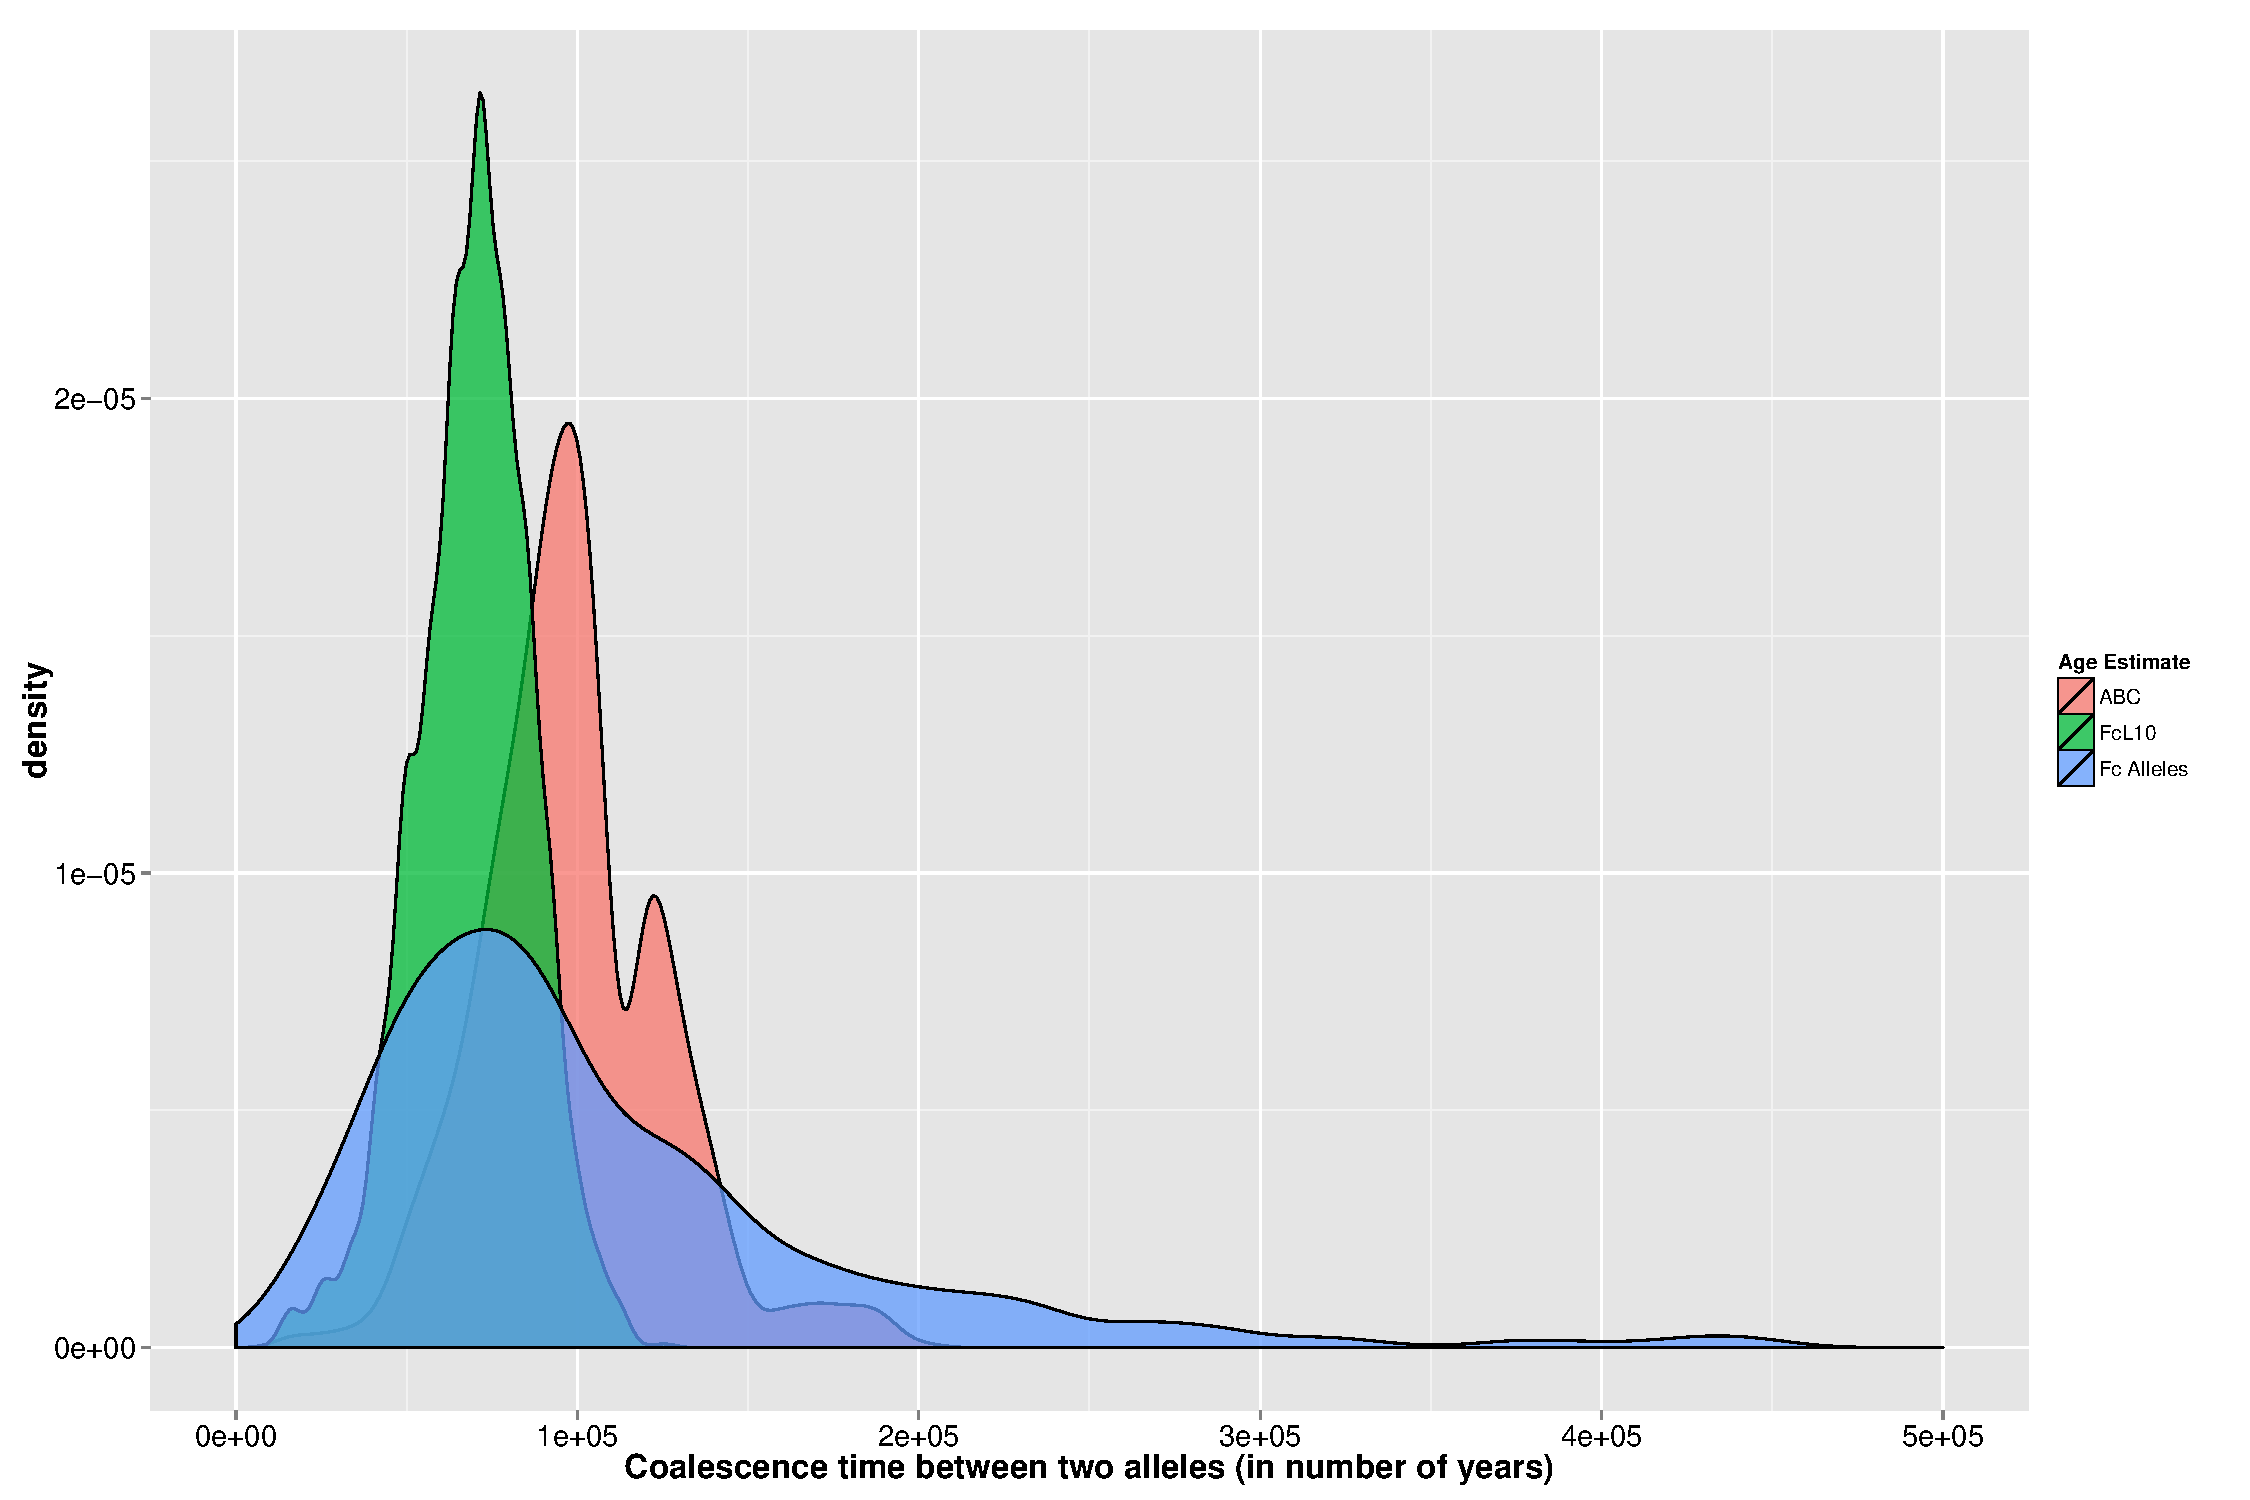
\includegraphics{Figures/Fcylindrus/DatesComparrisonMax}
\caption{Smoothed density plot of the maximum coalescence times (in generations) calculated for allelic pairs of the ABC Iron Transporter (red), Large Ribosomal Subunit (green) and allelic pairs from the genome (blue).\label{fig:FC_Res_1}}
\end{figure}

\subsection{Testing for recombination in the PCR amplified alleles with the PHI-test}

PHI – Scores calculated for the sequences of the ABC Iron transporter and the Large Ribosomal Subunit (Table \ref{table:Phitable}), and Figure \ref{fig:FC_Res_2} shows the refined incompatibility matrices between informative sites computed for the ABC Iron Transporter (A.), and the Large Ribosomal Subunit (B.). 
Yellow squares indicate pairs of informative sites that are compatible, darker squares indicate a pair of sites that are incompatible.
The presence of incompatible sites in these sequences, and the PHI-Scores and NSS scores shown in Table \ref{table:Phitable} suggests recombination has indeed affected these sequences.

\begin{figure}
\centering
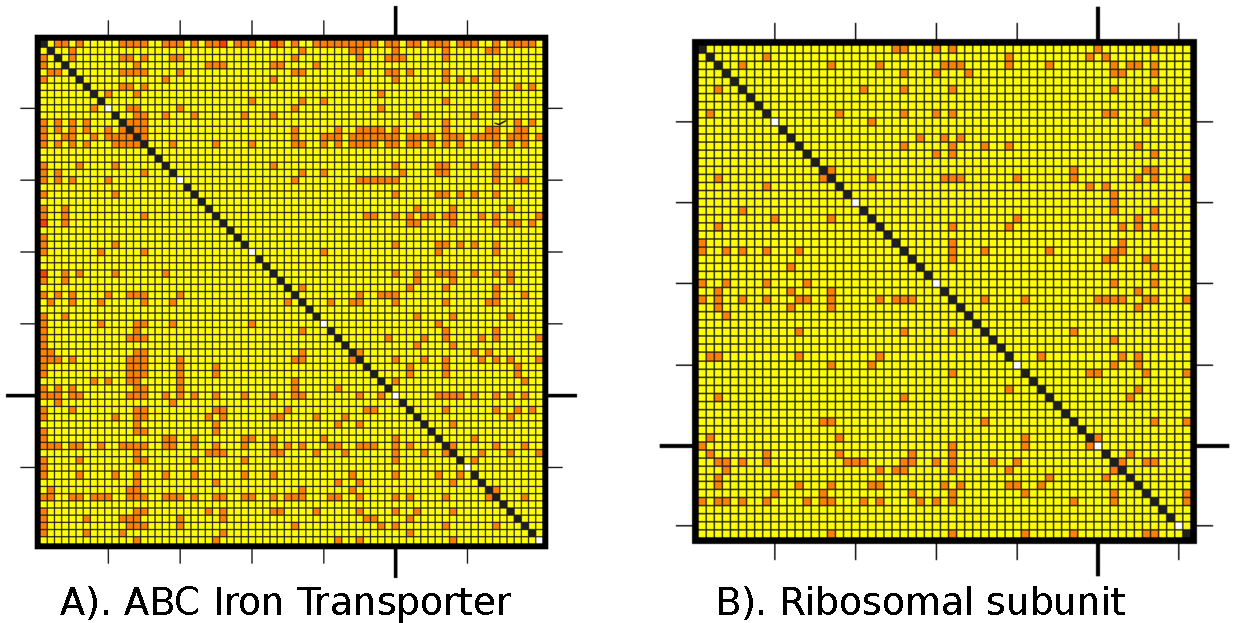
\includegraphics{Figures/Fcylindrus/matrices.pdf}
\caption{Incompatibility score matrices computed for A). The ABC iron Transporter and B). The Large Ribosomal Subunit.
Yellow boxes indicate two informative sites are compatible, and darker boxes indicate the two sites are incompatible.
The presence of incompatible sites in the alignments is suggestive of recombination.\label{fig:FC_Res_2}}
\end{figure}

\begin{table}
\centering
\caption{PHI-Score and Neighbor Similarity Scores of the PCR amplified sequences for three different window sizes.}
\begin{tabular}{ |P{2cm}|P{2cm}|P{2cm}|P{2cm}|P{2cm}|P{2cm}| }
 \hline
 Sequences & Window Size & PHI Score & P-Value & NSS & NSS P-Value \\
 \hline
 FeABC & 100 & 0.0930 & 0.0000405 & 0.81056 & 0.005 \\
 FeABC & 50 & 0.0955 & 0.0041100 & 0.81056 & 0.004 \\
 FeABC & 10 & 0.0870 & 0.0814000 & 0.81056 & 0.006 \\
 Fcl10 & 100 & 0.0930 & 4.0500000 & 0.81056 & 0.005 \\
 Fcl10 & 50 & 0.0385 & 0.0184000 & 0.88306 & 0.342 \\
 Fcl10 & 10 & 0.0500 & 0.2650000 & 0.88306 & 0.338 \\
 \hline
\end{tabular}
\label{table:Phitable}
\end{table}

\subsubsection{Comparative analysis of phylogenetic networks}

Figure \ref{fig:asexnet}. Shows an example network generated from sequences produced by the population genetics simulation scenario, in which individuals reproduced by asexual (clonal) reproduction.
This network is clearly characterized by two distinct clades, separated by long branches.

\begin{figure}
\centering
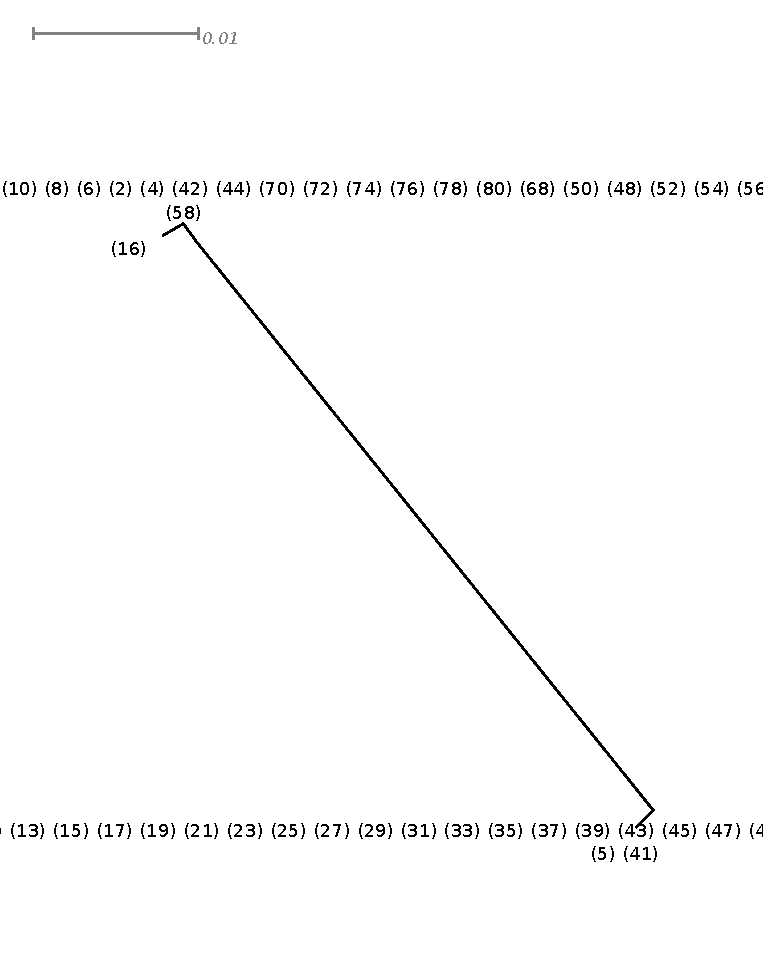
\includegraphics[width=\textwidth,keepaspectratio]{Figures/Fcylindrus/Asexual_randomSub}
\caption{Network of simulated allelic pairs, evolved under an asexual reproduction scheme.
The first copies of each allelic pair form a clade, and the second copies of each allelic pair form a clade.
This is because there is no recombination during gamete formation, as with clonal reproduction, offspring are clones of their parent.\label{fig:asexnet}}
\end{figure}

If \textit{F. cylindrus} has a history of asexual reproduction and ancient allelic divergence, then it is expected that the networks calculated for the PCR amplified sequences of the ABC Iron Transporter and the Large Ribosomal Subunit will have a similar structure to that of the network in Figure \ref{fig:asexnet}.

\begin{figure}
\centering
\subfigure[ABC Iron Transporter]{
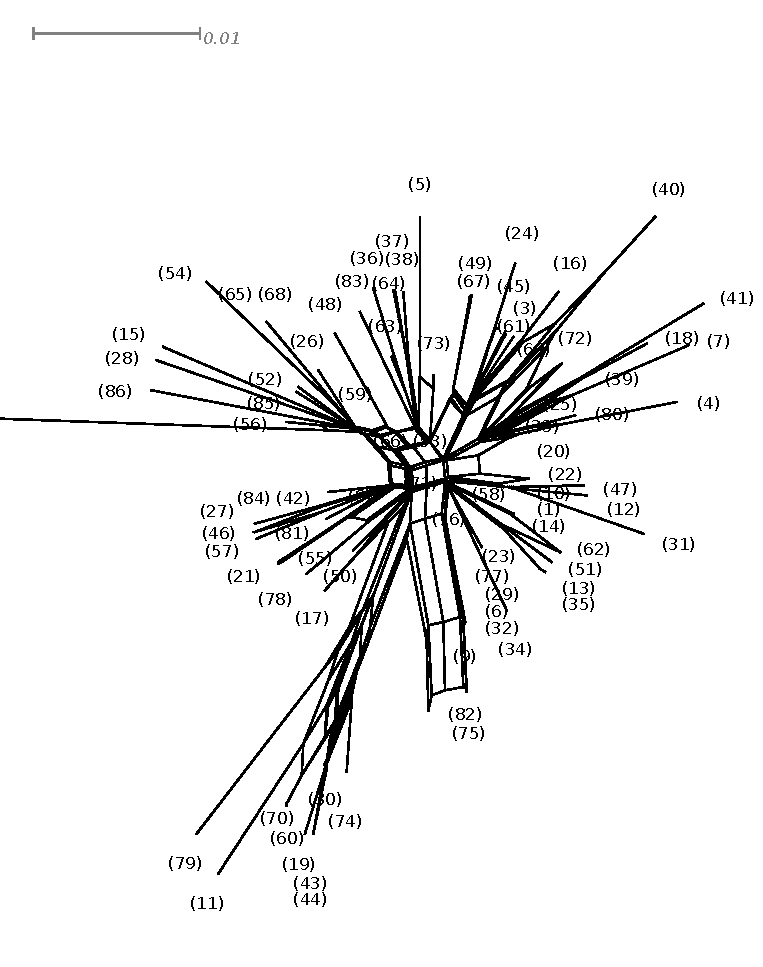
\includegraphics[width=0.5\textwidth]{Figures/Fcylindrus/3rd_Codon_Position_FC_ABC_IronTransporter}
}\\
\subfigure[Large Ribosomal Subunit]{
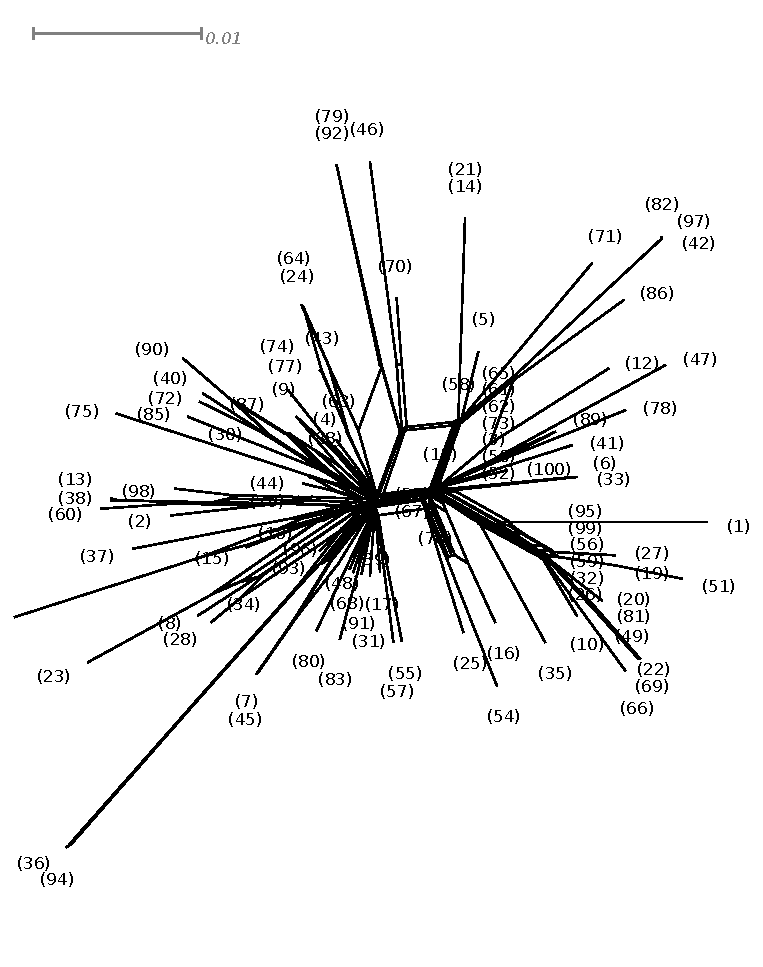
\includegraphics[width=0.5\textwidth]{Figures/Fcylindrus/3rd_Codon_Position_Fcl}
}
\caption{Split Networks of the ABC Iron Transporter and Ribosomal Subunit sequences have average branch lengths close to $10^{-2}$ and contain $~225$ splits. \label{fig:realnets}}
\end{figure}

Panels a and b in Figure \ref{fig:realnets} show the phylogenetic networks calculated for the PCR amplified sequences of the ABC Iron Transporter (a), and the Large Ribosomal Subunit (b).
These two networks are clearly different qualitatively to the kind of network in Figure \ref{fig:asexnet} that would be expected if \textit{F. cylindrus} had a history of asexual reproduction without meiotic recombination.
They do not show a clear partition between two clades or clusters, instead they have average branch lengths of around $0.1$, and contain around $255$ splits. 

\begin{figure}
\centering
\subfigure[The effect of $\theta$ on network branch lengths]{
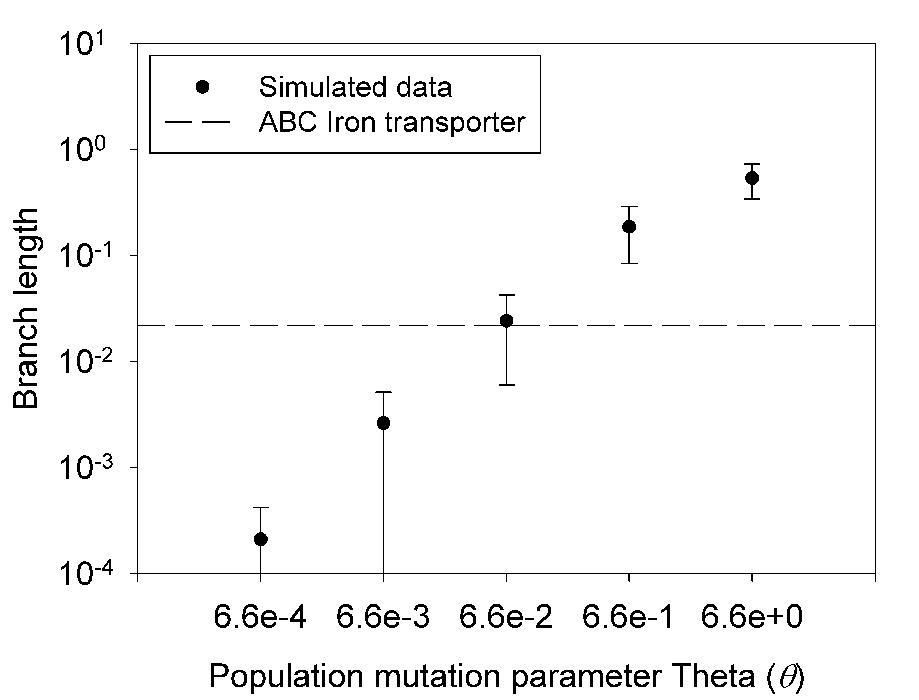
\includegraphics[width=0.8\textwidth]{Figures/Fcylindrus/branchlengths}
}\\
\subfigure[The effect of recombination rate on splits]{
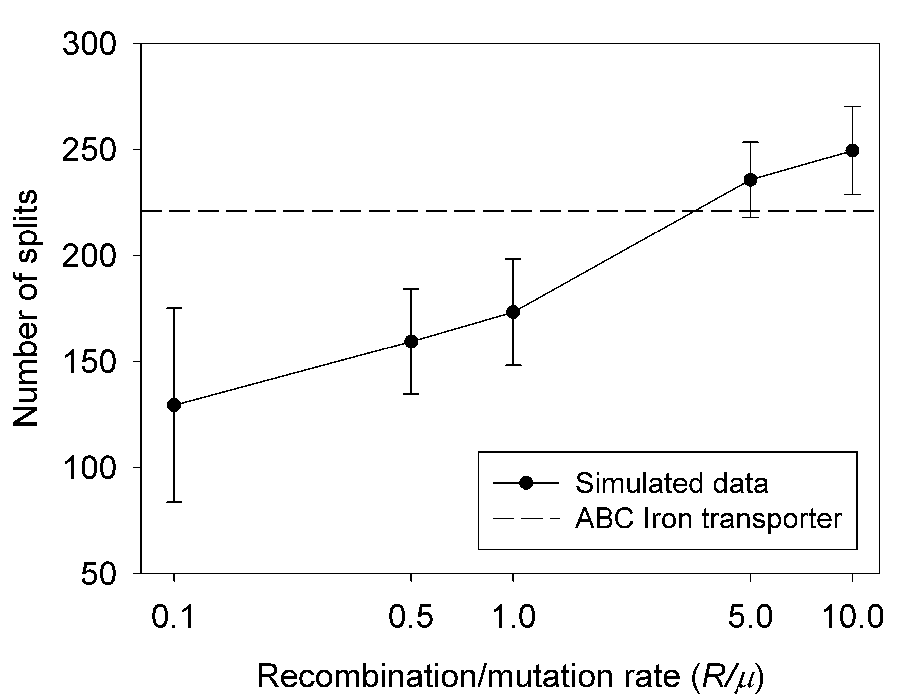
\includegraphics[width=0.8\textwidth]{Figures/Fcylindrus/splitsrmu}
}
\caption{Quantifying the branch lengths and number of splits in networks produced from simulations with varying levels of recombination and values of $\theta$.
Larger values of $\theta$ cause longer branches (a), and higher recombination rates result in more splits (b).\label{fig:relgraphs}}
\end{figure}

Panel a of Figure \ref{fig:relgraphs}, demonstrates the effect of increasing or decreasing $\theta$ in population genetic simulations, on the resulting sequences, and thus the networks produced:
The average branch lengths in networks, is positively related to the $\theta$ parameter set in the simulation.

\begin{figure}
\centering
\subfigure[$\theta = 0.66$]{
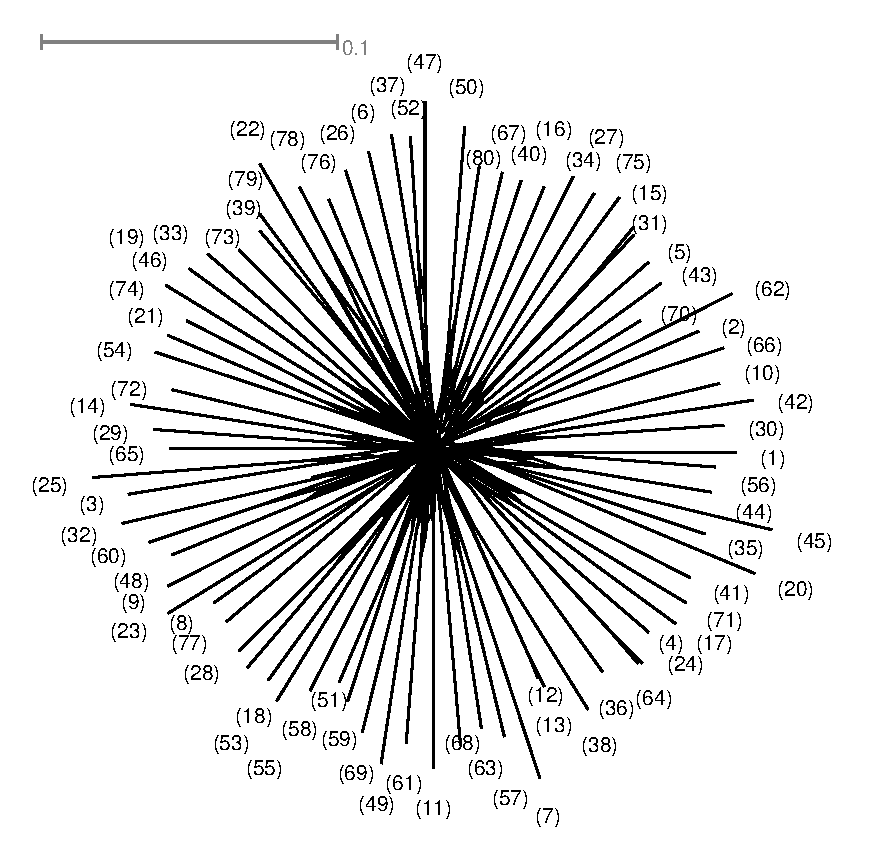
\includegraphics[width=0.5\textwidth]{Figures/Fcylindrus/Theta0_66Net}
}
\subfigure[$\theta = 0.066$]{
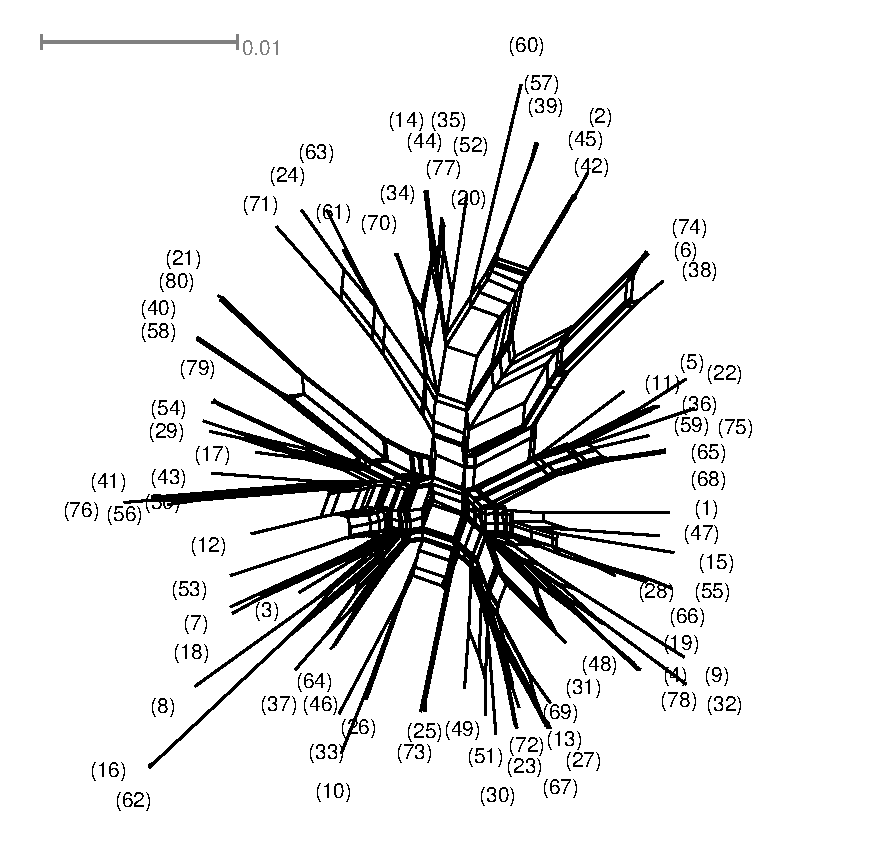
\includegraphics[width=0.5\textwidth]{Figures/Fcylindrus/Theta0_066Net}
}
\subfigure[$\theta = 0.0066$]{
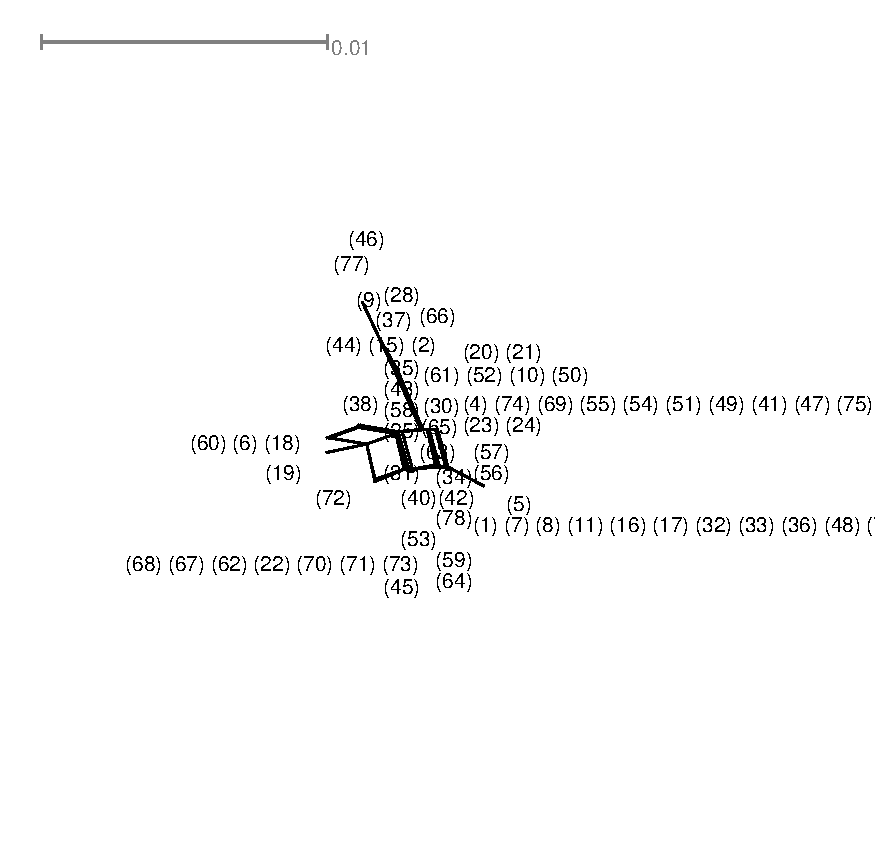
\includegraphics[width=0.5\textwidth]{Figures/Fcylindrus/Theta0_0066Net}
}
\caption{Networks computed from simulations with three different values of $\theta$.
Larger values of $\theta$ result in longer outer branches of networks.\label{fig:blnets}}
\end{figure}

Figure \ref{fig:blnets} presents this relationship qualitatively with the networks produced by Splitstree.
From figures \ref{fig:relgraphs} and \ref{fig:blnets} it can be seen that the networks best matching the real sequence networks (figure \ref{fig:realnets}) in terms of branch lengths, are those produced by simulations where $\theta = 0.066$, which is close to the value which LAMARC has estimated. 

Panel b of figure \ref{fig:relgraphs} demonstrates the effect of varying the recombination rate relative to the mutation rate in population genetic simulations, on the sequences and networks produced: The number of splits in networks is positively related to the recombination rate, relative to the mutation rate. This relationship is shown qualitatively in the networks drawn in figure \ref{fig:splitnets}.

\begin{figure}
\begin{center}
\subfigure[$R/\mu=1$]{
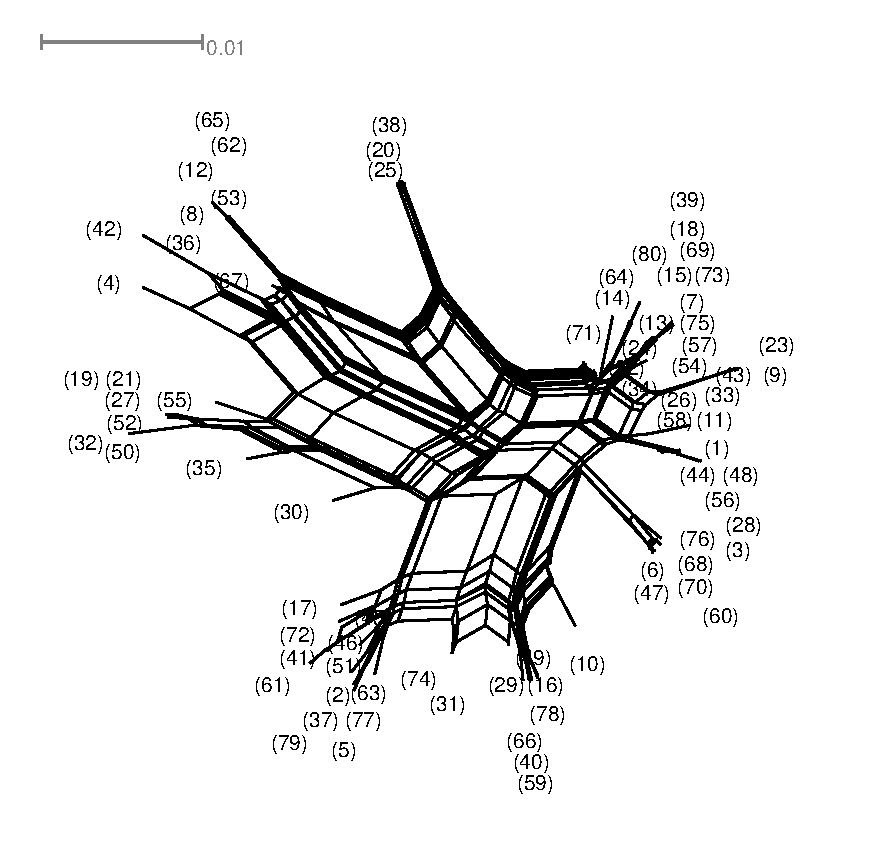
\includegraphics[width=0.5\textwidth]{Figures/Fcylindrus/rmuNet}
}
\subfigure[$R/\mu=5$]{
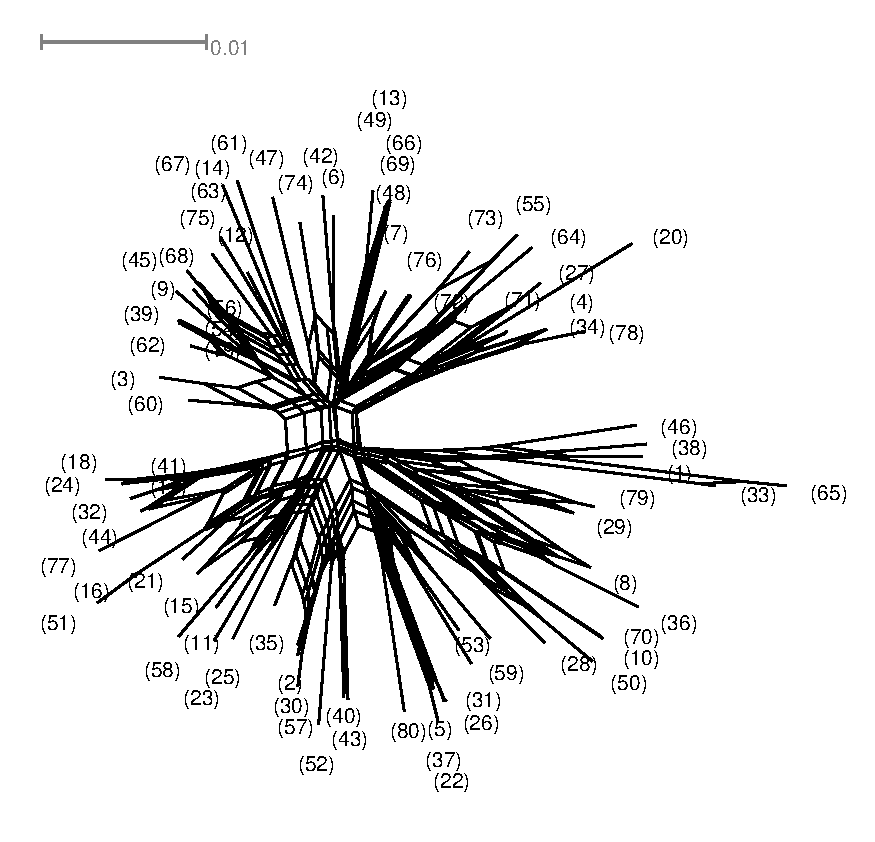
\includegraphics[width=0.5\textwidth]{Figures/Fcylindrus/rmu5Net}
}
\subfigure[$R/\mu=10$]{
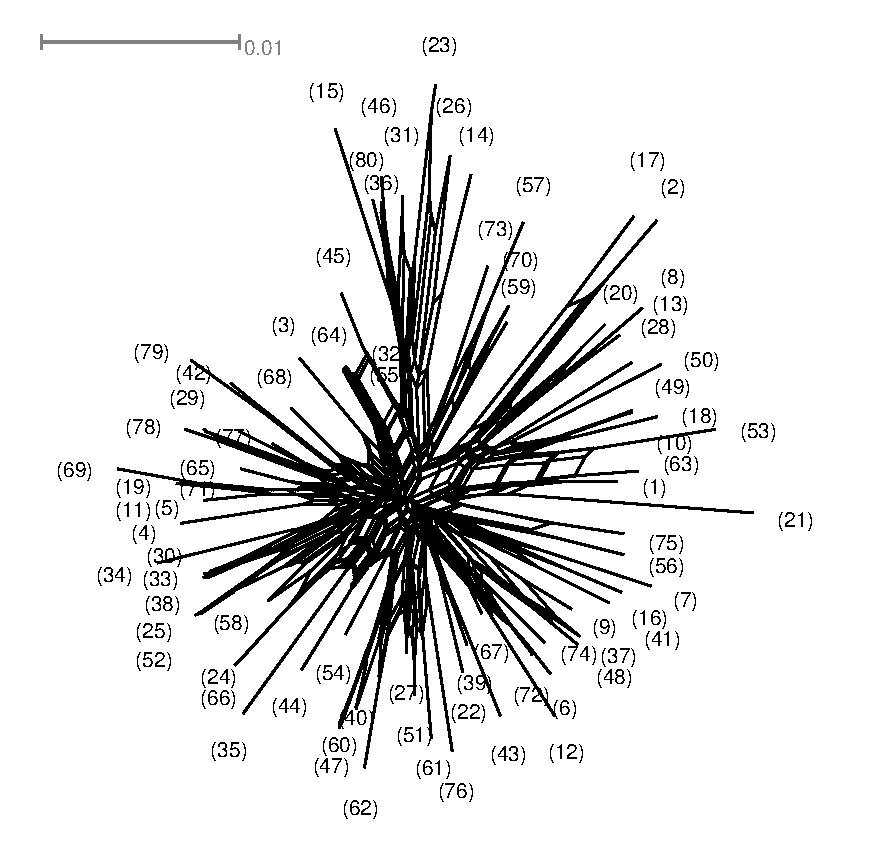
\includegraphics[width=0.5\textwidth]{Figures/Fcylindrus/rmu10Net}
}
\caption{Networks computed from simulations with three different levels of recombination, relative to the mutation rate $\mu$.
Larger values of $R$ result in more splits in networks.\label{fig:splitnets}}
\end{center}
\end{figure}





\section{Discussion}

The phylogenetic networks resulting from population genetic simulations support several assumptions we had about how recombination, and population mutation rate ($\theta$) may be inferred from phylogenetic networks.
Specifically, (1) the levels of Theta affect the average branch lengths of the networks, and (2) the extent of recombination affects the number of splits in phylogenetic networks.
These two assumptions are not controversial: a higher population mutation rate leads to more mutations in a population the same amount of time, and thus would lead to longer branches in any phylogeny or network computed for sequences sampled from the population \parencite{Frankham1996,Hein2004,Wakeley2008}.
Phylogenetic Split Networks \parencite{Huson1998} were conceived of as a way to detect and represent reticulate evolution.
Wherever there is a non-tree like structure or “loops”, recombination may be inferred.
The networks resulting from the simulations confirm these assumptions, and so give confidence in any inferences made about the population and evolution of \textit{F. cylindrus} from the networks of the ABC Iron Transporter sequences, and the Large Ribosomal Subunit Sequences.

Secondly, from comparisons between the networks of the ABC Iron Transporter sequences, Large Ribosomal Subunit Sequences, and simulated networks, it was concluded that LAMARC \parencite{Kuhner2006a} estimate of $\Theta$ was a reasonable estimate for the population of \textit{F. cylindrus}.
It was also concluded that these networks provide evidence of recombination for the sequences of the ABC Iron Transporter, and in the sequences of the Large Ribosomal Subunit.
Evidence of recombination does not have to mean that an organism is reproducing sexually, meiotic recombination is associated with sexual reproduction, but mitotic recombination could also explain the recombination signal detected in these sequences.
However, whilst mitotic or meiotic recombination may explain the recombination signal in the sequences, it was concluded that ancient asexuality is not a likely explanation, because of the lack of similarity of the ABC Iron Transporter, and the Large Ribosomal Subunit networks, to the networks generated by simulations of ancient asexual evolution.


\subsection{Sex and the diatom reproductive cycle}

Even though sexual reproduction has not been observed in the lab cultures of \textit{F. cylindrus}, this diatom does not appear to be an ancient asexual.
This might not be surprising given what is already known about Diatom biology and sexual reproduction.
The typical cell cycle of Diatoms is diplontic i.e. the vegetative cells are diploid, and the haploid gametes are short lived \parencite{Chepurnov2004}.

The Diatom life cycle features two key phases which may be summarized by the following:

The first phase is a long vegetative phase; this phase can last for months or years. During this phase, vegetative cells divide by mitosis, gradually becoming smaller. 
The cell size decrease during the vegetative phase of the diatom life cycle is due to the shape and structure of Diatom cell walls and the division pattern of the Diatoms. 
The cell wall is made of sillicated components, which together are termed the frustule. The frustule is made of two overlapping halves or thecae \parencite{Chepurnov2004,Davidovich1998,Poulickova2008}.
These thecae are not the same size, the larger of the two thecae is called the epitheca, and the smaller of the two is called the hypotheca.
When mitosis occurs, cytokinesis splits the diatom where the two thecae overlap.
The two resulting daughter cells inherit one of the parent cell’s two thecae as its own epitheca, and they grow their own hypotheca \parencite{Chepurnov2004}.
Since one of the daughter cells inherits a hypotheca as it epitheca, it will be smaller in size to its parent cell.
Thus the average cell size of a population of diatoms decreases as mitotic cell division occurs.

The second phase is shorter, and includes sexual reproduction and the production of new vegetative cells, restoring the cell size \parencite{Chepurnov2004}.
Production of gametes during the sexual reproduction phase has been demonstrated to occur by classical meiosis in many Diatom species.
Diatoms restore their cell size through the production of auxospores, which result from sexual reproduction \parencite{Davidovich1998}.
During auxosporulation, recombination and cell size restitution occurs: gametes fuse to form the auxospore, which expands and a new cell is produced within.
The cell walls of the gamete producing cells are lost, and so the auxospore must then form the shape of the vegetative cells de novo \parencite{Chepurnov2004}.
If a population of Diatom cells did not undergo sexual reproduction to produce the auxospores to restore their cell size, the population would gradually decrease in cell size until they become critically small.
At this point the population would die, and this has been observed in experimental cultures.
Diatom cells can only become sexualized when they are sufficiently small, but they may also not be able to become sexualized if they become too small or hit the critical cell size before they die \parencite{Chepurnov2004,Davidovich1998,Poulickova2008}.
The maximum size of initial diatom cells, the maximum and minimum sizes of cells capable of sexual reproduction, and the minimum size before death are strict for each diatom species and are termed cardinal points \parencite{Chepurnov2004}.

However, despite the role of sex in the restoration of cell size in diatoms, it is not always necessary for cell size restoration.
For some diatom species, asexual auxosporulation is a possibility, presumably it is some secondary modification of a developmental pathway that was sexual, and some species do not even undergo auxosporulation and exist as entirely as asexual populations, and their cell size is restored by vegetative cell enlargement \parencite{Chepurnov2004,Gallagher1983,Nagai1995,Sabbe2004,werner1977biology}.
Species such as \textit{Caloneis amphisbaena} and \textit{Sellaphora pupula} "lanceolate" have been found to exist in populations of a very limited range of cell size, and this cell size has remained unchanged after many generations of observation \parencite{Mann1989,Mann2004}.

Therefore, whilst sex is a common feature of the diatom life cycle, and is important for cell size restoration in many species, it is not unreasonable to suggest the hypothesis that a diatom like \textit{F. cylindrus} could have evolved asexually for a long period of time.
However, the network reconstructions and evidence of recombination demonstrated by this study cast doubt on that hypothesis as an explanation for the diverged alleles.


\subsubsection{Allelic Divergence in diatoms may be explained by population size}

If the “ancient asexuality hypothesis” is rejected as the explanation of the diverged alleles in \textit{F. cylindrus}, then an alternative explanation of how this diatom evolved diverged and functionally differentiated alleles is desired.
These alleles show signatures of positive selection, and they are differentially expressed.
The question is; assuming sexual reproduction and recombination, why does recombination not homogenize the sequence variation between two alleles over time? 

An alternative hypothesis explaining the adaptive evolution of \textit{F. cylindrus} is a large population size, which would lead to bigger coalescence times between maternal and paternal loci.
In combination with a low recombination rate, this would result in independent adaptive evolution and divergence of the different haplotypes.
This is intuitive if one considers a coalescent process back through time of an idealized population, because the coalescent relates genetic diversity to demographic history.
In such a process, the probability that any two lineages extant at time $t$, coalesce in the previous generation $t – 1$, is the probability that they share a parental DNA sequence.
For a diploid population there are $2N_e$ alleles in every generation, assuming a constant population size \parencite{Hein2004}.
Assuming random mating and neutral evolution, the probability any two alleles coalesce in the previous generation (i.e. they share the same parental sequence) is $1 / (2N_e)$.
Therefore, the probability those two alleles do not coalesce, is $1 – (1/(2N_e))$.
These probabilities are dependent on the size of the population in question \parencite{Wakeley2008}.
Larger populations, result in a smaller probability that two alleles coalesce in the previous generation, and a greater probability that they do not.
With each successive previous generation, the probability of coalescence is geometrically distributed \parencite{Hein2004,Wakeley2008}.
This means that it is the product of coalescence at the generation of interest and the probability of non-coalescence at the preceding generations i.e.
\begin{equation}
P_c(t)=\bigg(1-\frac{1}{2N_e}\bigg)^{t-1}\bigg(\frac{1}{2N_e}\bigg)
\end{equation}
From this equation, it can be seen that with larger populations, the probability that two alleles coalesce further back in time is greater i.e. the expected coalescence time between two alleles is larger, therefore alleles are expected to be more diverged.

This explanation is consistent with the estimation of a $\Theta$ of 0.066 by the LAMARC \parencite{Kuhner2006a} analysis, which is also supported by the simulations.
The population mutation rate $\Theta$, is proportional to the product of the mutation rate and the effective population size and so the value predicted by LAMARC could be the result of a very large population.
Furthermore, prior research has been performed to estimate the abundance of \textit{F. cylindrus} in water columns around the Antarctic \parencite{Kang1992}.
During the summer, numbers of $7.9 \times 10^{10}$ cells $^{m-2}$ were observed, and during the winter, numbers of $1.1 \times 10^8$ cells $^{m-2}$ were observed.
Marginal ice zones are known to be sites with much dynamic activity such as jets, eddies, currents, melting, freezing, and upwelling \parencite{Kang1992}.
They are also known to be sites of increased phytoplankton biomass and primary productivity, due to their light levels, ice-distribution, and vertical stability.

Therefore, the hypothesis that a large population size explains the levels of diversity is consistent with both population genetic (coalescent) theory, results of this study, as well as the findings of other research.
It is also attractive, because of its simplicity.
It is much more plausible that a phytoplankton species has very large populations; than it is that the species had abandoned sex as a reproductive strategy:
Sex is a common aspect of the diatom life cycle and is often essential for cell size restoration and population survival.
Furthermore, as was explored in the Introduction, there is a substantial body of theory explaining why sexual reproduction evolved two become a widespread reproductive strategy, and is advantageous, despite the apparent costs.


\subsubsection{Study limitations and subsequent FALCON assembly}
However, this study has some limitations which should be acknowledged when considering these results.
First, whilst evidence of recombination in the form of the splits networks and the presence of incompatible sites is obtained from these sequences, it was not possible to examine any larger recombination events or blocks as was possible for \textit{Albugo candida} in chapter \ref{chap:Acandida}.
Indeed, the number of informative sites was too small for the HybridCheck software (which was implemented to analyse large contigs) to effectively run.
Secondly, the analyses were only performed on two genes.
Whilst it was concluded that the two genes were representative of the larger set of diverged alleles (figure \ref{fig:FC_Res_1}), we do not know if the PCR primers amplified only maternal and paternal alleles of those genes or if some of the sequences amplified also represent paralogues.

The question of whether the diverged alleles observed in the assembly were truly diverged alleles was resolved for the assembly described in the introduction experimentally.
Single haplotyped fosmids were Sanger sequenced by collaborators, providing contiguity information and they were compared with the assembled genomic scaffolds, and an annotated protein set from the diverged regions in the genome.
Data from these comparisons revealed a clear separation between allelic pairs and gene duplications based on 100\% identity to the haplotyped Sanger sequenced fosmids.
Additionally, the nucleotide similarity of the diverged alleles (mean = $97.01 \pm 0.03\%$) is significantly (p-value $< 10^{-09}$) higher than for gene duplicates (mean = $84.07 \pm 0.36\%$). 
Therefore, whilst it may be that some uncollapsed regions of the assembly could be duplicates, there is high confidence that the allelic pairs identified are indeed diverged alleles and not duplicates.

Since this work has been completed, an assembly has been completed using PacBio long read sequencing technology, which has also supported that true diverged alleles have been identified and that they are not duplicated sequences (although duplicated sequences are indeed present in the genome). 
The sequencing work and library preparation was completed by the platforms and pipelines team.
A 20kb fragment length library was constructed, and a 4kb insert size library was also created. 
Both libraries were sequences using the PacBio RS2 instrument, using SMRT cells with the c4P6 chemistry.
The 20kb fragment length library yielded 1.37Gb of data, and the 4kb insert size library yielded 3.85Gb of data.
The final N50 of read length varied between 8215 to 8898bp for the 20kb fragment length library, and the N50 ranged from from 2558 to 2680bp for the 4kb insert size library.

Assembly was completed by collaborator Pirita Paajanen, who combined the data from the SMRT cells and filtered the shortest reads, yielding 3.8Gb of data which gave 63x coverage.
Assembly was completed using the diploid aware PacBio assembler, Falcon 0.3.0.
The output of the Falcon assembler was divided into two parts.
The haploid assembly resulted in primary contigs from which a genome size of 59.7Mb was deduced. 
However, the assembler also produced alternate contigs which were the result of the assembler being unable to decide between two possible routes through the genome graph the genome.
Such 'bubbles' in the genome graph represent diverged haplotypes, containing diverged alleles.

The haplotype divergence differed between chromosomes: The longest chromosome 000000F had only one alternate contig with a length of 6047bp.
In contrast, contig 000002F was 1246645bp long and had 14 associated alternative contigs, of a total sequence length of 633764bp.
For each of the 14 alternative contigs of chromosome 000002F, I extracted and aligned the two haplotype sequences using the pairwise alignment algorithm available in the Bio.jl software package (https://biojulia.github.io/Bio.jl), using an EDNA scoring matrix.
Once aligned, a non-overlapping sliding window was moved across the sequences, and the p-distance between the sequences within each window was calculated. For each computation, the width of the sliding window was set as 1\% of the width of the pairwise alignment in (bp).
The results of this analysis are included as extra information in the appendix, figure \ref{fig:falconwindows}.
The figure demonstrates different levels of divergence across the diverged haplotype pairs, including the appearance of indels between some haplotype pairs.
Further work will show how the sequences of allelic pairs align to the FALCON assembly, revealing which pairs align to different haplotypes of a FALCON 'bubble' (true allelic pairs), and which pairs align to the same haplotype of a FALCON 'bubble' (potentially gene duplicates).

At the time of writing, multiple population samples of \textit{F. cylindrus} are not available, and so analyses presented here used sequences from cultures, and so further population genetic analyses should be conducted in the future as more data becomes available, for example to assess the population structure of \textit{F. cylindrus} and investigate if gene flow is occurring between subpopulations of \textit{F. cylindrus}.

The fact that the genome assembly contains some duplicates, and that some of the allelic pairs analysed in this study may be found to be duplicates is not problematic for the hypothesis that this Diatom species has adapted through alleleic divergence, as it may be argued allelic divergence could lead to gene duplication and the conditions for the divergence of alleles and the divergence of duplicates overlap: 
When diverged alleles are maintained in a population due to heterozygote advantage, duplications may rapidly spread through the population, causing an individual to act as a genetic heterozygote yet still breed true.
\cite{Proulx2006} argued that genetic redundancy is the mechanism usually cited as allowing duplicate genes to diverge, but redundancy is present in a diploid before duplication: Dominance creates the same kind of redundancy duplicates have, but for alleles of single copy genes.
Therefore mode of inheritance is the thing then which most distinguishes duplicates from single copy genes: Segregation prevents the fixed inheritance of alternative allelic variants at a single locus \parencite{Proulx2006}.
In other words, heterozygotes at one locus are broken up by segregation during sexual reproduction, whereas duplicate loci in an individual can carry copies of alternate alleles at different loci.
Their results show that fitness relationships that allow divergent alleles to evolve at one locus overlap significantly with those that allow the divergence of previously duplicated genes at two different loci \parencite{Proulx2006}.


\subsubsection{Conclusion}

The genome of the polar diatom \textit{Fragilariopsis cylindrus} contains diverged alleles that are differentially expressed in different environmental conditions.
Evidence of recombination was found which contradicts the ancient asexuality hypothesis explaining how these diverged alleles may have evolved.
An alternative, competing hypothesis is proposed, supported by the evidence presented, that a large population size has allowed diversifying selection to differentiate the alleles of genes despite the homogenizing effect of recombination.
Additional population samples, and analysis of larger contigs made possible by improved genome assembly for recombination, will help answer the question of how \textit{F. cylindrus} has evolved this remarkable strategy to cope with varying environmental conditions.



